\documentclass[11pt, oneside]{book}

%%%%%%%%%%%%%%Include Packages%%%%%%%%%%%%%%%%%%%%%%%%%%
\usepackage{xcolor}
\usepackage{mathtools}
\usepackage[a4paper, total={6in, 8in}, margin=1.25in]{geometry}
\usepackage{amsmath}
\usepackage{amssymb}
\usepackage{paralist}
\usepackage{rsfso}
\usepackage{amsthm}
\usepackage{wasysym}
\usepackage[inline]{enumitem}   
\usepackage{hyperref}
\usepackage{tocloft}
\usepackage{wrapfig}
\usepackage{titlesec}
\usepackage{colortbl}
\usepackage{stackengine} 
\usepackage{listings}
%%%%%%%%%%%%%%%%%%%%%%%%%%%%%%%%%%%%%%%%%%%%%%%%%%%%%%%%



%%%%%%%%%%%%%%%Code%%%%%%%%%%%%%%%%%%%%%%%%%%%%%%%%%%%%%
\definecolor{codegreen}{rgb}{0,0.6,0}
\definecolor{codegray}{rgb}{0.5,0.5,0.5}
\definecolor{codepurple}{rgb}{0.58,0,0.82}
\definecolor{backcolour}{rgb}{0.95,0.95,0.92}

\lstdefinestyle{mystyle}{
    backgroundcolor=\color{backcolour},   
    commentstyle=\color{codegreen},
    keywordstyle=\color{magenta},
    numberstyle=\tiny\color{codegray},
    stringstyle=\color{codepurple},
    basicstyle=\ttfamily\footnotesize,
    breakatwhitespace=false,         
    breaklines=true,                 
    captionpos=b,                    
    keepspaces=true,                 
    numbers=left,                    
    numbersep=5pt,                  
    showspaces=false,                
    showstringspaces=false,
    showtabs=false,                  
    tabsize=2
}
%%%%%%%%%%%%%%%%%%%%%%%%%%%%%%%%%%%%%%%%%%%%%%%%%%%%%%%%

%%%%%%%%%%%%%%%Chapter Setting%%%%%%%%%%%%%%%%%%%%%%%%%%
\definecolor{gray75}{gray}{0.75}
\newcommand{\hsp}{\hspace{20pt}}
\titleformat{\chapter}[hang]{\Huge\bfseries}{\thechapter\hsp\textcolor{gray75}{$\mid$}\hsp}{0pt}{\Huge\bfseries}
%%%%%%%%%%%%%%%%%%%%%%%%%%%%%%%%%%%%%%%%%%%%%%%%%%%%%%%%

%%%%%%%%%%%%%%%%%Theorem environments%%%%%%%%%%%%%%%%%%%
\newtheoremstyle{break}
  {\topsep}{\topsep}%
  {\itshape}{}%
  {\bfseries}{}%
  {\newline}{}%
\theoremstyle{break}
\theoremstyle{break}
\newtheorem{axiom}{Axiom}
\newtheorem{thm}{Theorem}[section]
\renewcommand{\thethm}{\arabic{section}.\arabic{thm}}
\newtheorem{lem}{Lemma}[thm]
\newtheorem{cor}{Corollary}[thm]
\newtheorem{defn}{Definition}[thm]
\newenvironment{indEnv}[1][Proof]
  {\proof[#1]\leftskip=1cm\rightskip=1cm}
  {\endproof}
%%%%%%%%%%%%%%%%%%%%%%%%%%%%%%%%%%%%%%%%%%%%%%%%%%%%%%


%%%%%%%%%%%%%%%%%%%%%%%Integral%%%%%%%%%%%%%%%%%%%%%%%
\def\upint{\mathchoice%
    {\mkern13mu\overline{\vphantom{\intop}\mkern7mu}\mkern-20mu}%
    {\mkern7mu\overline{\vphantom{\intop}\mkern7mu}\mkern-14mu}%
    {\mkern7mu\overline{\vphantom{\intop}\mkern7mu}\mkern-14mu}%
    {\mkern7mu\overline{\vphantom{\intop}\mkern7mu}\mkern-14mu}%
  \int}
\def\lowint{\mkern3mu\underline{\vphantom{\intop}\mkern7mu}\mkern-10mu\int}
%%%%%%%%%%%%%%%%%%%%%%%%%%%%%%%%%%%%%%%%%%%%%%%%%%%%%%



\newcommand{\R}{\mathbb{R}}
\newcommand{\N}{\mathbb{N}}
\newcommand{\Z}{\mathbb{Z}}
\newcommand{\Q}{\mathbb{Q}}
\newcommand{\C}{\mathbb{C}}
\newcommand{\T}{\mathcal{T}}
\newcommand{\M}{\mathcal{M}}
\newcommand{\Symm}{\text{Symm}}
\newcommand{\Alt}{\text{Alt}}
\newcommand{\Int}{\text{Int}}
\newcommand{\Bd}{\text{Bd}}
\newcommand{\Power}{\mathcal{P}}
\newcommand{\ee}[1]{\cdot 10^{#1}}
\newcommand{\spa}{\text{span}}
\newcommand{\sgn}{\text{sgn}}
\newcommand{\degr}{\text{deg}}
\newcommand{\pd}{\partial}
\newcommand{\that}[1]{\widetilde{#1}}
\newcommand{\lr}[1]{\left(#1\right)}
\newcommand{\vmat}[1]{\begin{vmatrix} #1 \end{vmatrix}}
\newcommand{\bmat}[1]{\begin{bmatrix} #1 \end{bmatrix}}
\newcommand{\pmat}[1]{\begin{pmatrix} #1 \end{pmatrix}}
\newcommand{\rref}{\xrightarrow{\text{row\ reduce}}}
\newcommand{\txtarrow}[1]{\xrightarrow{\text{#1}}}
\newcommand\oast{\stackMath\mathbin{\stackinset{c}{0ex}{c}{0ex}{\ast}{\Circle}}}
\newcommand{\txt}{Wald's \textit{General Relativity}}

\newcommand{\note}{\color{red}Note: \color{black}}
\newcommand{\remark}{\color{blue}Remark: \color{black}}
\newcommand{\example}{\color{green}Example: \color{black}}
\newcommand{\exercise}{\color{green}Exercise: \color{black}}

%%%%%%%%%%%%%%%%%%%%%%Roman Number%%%%%%%%%%%%%%%%%%%%%%%
\makeatletter
\newcommand*{\rom}[1]{\expandafter\@slowromancap\romannumeral #1@}
\makeatother
%%%%%%%%%%%%%%%%%%%%%%%%%%%%%%%%%%%%%%%%%%%%%%%%%%%%%%%%%

%%%%%%%%%%%%%table of contents%%%%%%%%%%%%%%%%%%%%%%%%%%%%
%\setlength{\cftchapindent}{0em}
%\cftsetindents{section}{2em}{3em}
%
%\renewcommand\cfttoctitlefont{\hfill\huge\bfseries}
%\renewcommand\cftaftertoctitle{\hfill\mbox{}}
%
%\setcounter{tocdepth}{2}
%%%%%%%%%%%%%%%%%%%%%%%%%%%%%%%%%%%%%%%%%%%%%%%%%%%%%%%%%%


%%%%%%%%%%%%%%%%%%%%%Footnotes%%%%%%%%%%%%%%%%%%%%%%%%%%%
\newcommand\blfootnote[1]{%
  \begingroup
  \renewcommand\thefootnote{}\footnote{#1}%
  \addtocounter{footnote}{-1}%
  \endgroup
}
%%%%%%%%%%%%%%%%%%%%%%%%%%%%%%%%%%%%%%%%%%%%%%%%%%%%%%%%%

%%%%%%%%%%%%%%%%%%%%%Section%%%%%%%%%%%%%%%%%%%%%%%%%%%%%
\makeatletter
\def\@seccntformat#1{%
  \expandafter\ifx\csname c@#1\endcsname\c@section\else
  \csname the#1\endcsname\quad
  \fi}
\makeatother
%%%%%%%%%%%%%%%%%%%%%%%%%%%%%%%%%%%%%%%%%%%%%%%%%%%%%%%%%

%%%%%%%%%%%%%%%%%%%%%%%%%%%%%%%%%%%Enumerate%%%%%%%%%%%%%%
\makeatletter
% This command ignores the optional argument 
% for itemize and enumerate lists
\newcommand{\inlineitem}[1][]{%
\ifnum\enit@type=\tw@
    {\descriptionlabel{#1}}
  \hspace{\labelsep}%
\else
  \ifnum\enit@type=\z@
       \refstepcounter{\@listctr}\fi
    \quad\@itemlabel\hspace{\labelsep}%
\fi}
\makeatother
\parindent=0pt
%%%%%%%%%%%%%%%%%%%%%%%%%%%%%%%%%%%%%%%%%%%%%%%%%%%%%%%%%%



\begin{document}

	\begin{titlepage}
		\begin{center}
			\vspace*{0.5cm}
			\Huge \color{red}
				\textbf{Homework 3}\\
			\vspace{0.5cm}			
			\Large \color{black}
			Physics 542 - Quantum Optics\\
			Professor Alex Kuzmich
			\vspace{1.5cm}

			
\includegraphics[scale=1.15]{hmm.pdf}
			
			
			\vspace{2cm}
			\LARGE
				\textbf{Jinyan Miao}\\
				\hfill\break
				\LARGE Fall 2023\\
			\vspace{1cm}

		\vspace*{\fill}
		\end{center}			
	\end{titlepage}

\chapter{}
Straightforward algebra leads to
\begin{align*}
-&\gamma(\hat{\sigma}_0 \hat{\rho} + \hat{\rho}\hat{\sigma}_0)+ \gamma_2 \hat{\sigma}_- \hat{\rho} \hat{\sigma}_+ + 2\Gamma\hat{\sigma}_0 \hat{\rho} \hat{\sigma}_0\\
&=
\bmat{0 & 0 \\0 & -\gamma}\bmat{\rho_{11} & \rho_{12} \\ \rho_{21} & \rho_{22}}+\bmat{\rho_{11} & \rho_{12} \\ \rho_{21} & \rho_{22}}
\bmat{0 & 0 \\0 & -\gamma}+
\bmat{0 & \gamma_2 \\ 0 & 0}
\bmat{\rho_{11} & \rho_{12} \\ \rho_{21} & \rho_{22}}
\bmat{0 & 0 \\ 1 & 0}
+
\bmat{0 & 0 \\ 0 & 2\Gamma}
\bmat{\rho_{11} & \rho_{12} \\ \rho_{21} & \rho_{22}}
\bmat{0 & 0 \\ 0 & 1}\\
&= 
\bmat{0 & 0\\ -\gamma\rho_{21} & -\gamma\rho_{22}} + 
\bmat{0 & -\gamma \rho_{12} \\ 0 & -\gamma \rho_{22}} + 
\bmat{\gamma_2 \rho_{21} & \gamma_2 \rho_{22} \\ 0 & 0}\bmat{0 & 0 \\ 1 & 0} + 
\bmat{0 & 0 \\ 2\Gamma \rho_{21} & 2\Gamma\rho_{22}} \bmat{0 & 0 \\ 0 & 1}\\
&= \bmat{0 & 0\\ -\gamma\rho_{21} & -\gamma\rho_{22}} + 
\bmat{0 & -\gamma \rho_{12} \\ 0 & -\gamma \rho_{22}} + 
\bmat{\gamma_2 \rho_{22} & 0 \\ 0 & 0} + \bmat{0 & 0 \\ 0 & 2\Gamma\rho_{22}}\\
&= \bmat{\gamma_2 \rho_{22} & -\gamma \rho_{12} \\ -\gamma\rho_{21} & -2\gamma \rho_{22}+ 2\Gamma \rho_{22}}\,.
\end{align*}

Comparing Eq.\ (3.31a) and (3.20a), the relaxation term in the $\dot{\rho}_{11}$ equation is $\gamma_2 \rho_{22}$, which agrees with the $(1,1)$-entry in the matrix computed. \\

Comparing Eq.\ (3.31b) and (3.20b), the relaxation terms in the $\dot{\rho}_{22}$ equation is $$-\gamma_2 \rho_{22} = -2(\gamma-\Gamma)\rho_{22} = -2\gamma \rho_{22}+2\Gamma\rho_{22} \,,$$ which agrees with the $(2,2)$-entry in the matrix computed. \\

Comparing Eq.\ (3.31c) and (3.20c), the relaxation term in the $\dot{\rho}_{12}$ equation is $-\gamma \rho_{12}$, which agrees with the $(1,2)$-entry in the matrix computed. \\

Comparing Eq.\ (3.31d) and (3.20d), the relaxation term in the $\dot{\rho}_{21}$ equation is $-\gamma \rho_{21}$, which agrees with the $(2,1)$-entry in the matrix computed. \\

These complete the derivation. 


\chapter{}
Here we solve the Bloch equations numerically for $\gamma = \gamma_2/2 = 1/2$, $\delta = 0.1$, and $|\Omega_0| \in \{0.2, 3\}$. The solution of $w$ is plot as a function of time, with initial condition $w(t=0) =\rho_{22}-\rho_{11} =-1$, that is the atom is initially in its ground state $\rho_{11} = 1$. 

\begin{center}
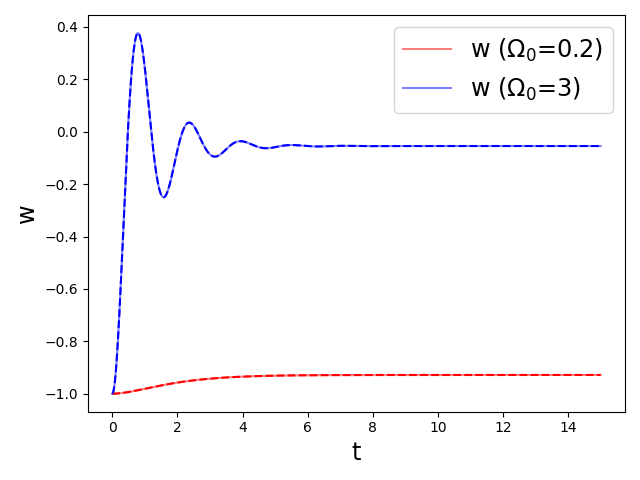
\includegraphics[scale=0.6]{542HW3/fig}
\end{center}

For comparison, the numerical solutions to the Bloch equations are plotted in solid curves, and the numerical solutions to Eq.\ (3.54) in \textit{Berman} are plotted in dashed curves. We see here the solid curves agree perfectly with the dashed curves. \\

We also conclude that the Bloch vector approach its steady-state
value monotonically in the case of $\Omega_0 = 0.2$ (plotted in red). \\

* \textit{The script for numerical computations is attached on the next page.}
\newpage
\lstset{style=mystyle}
\lstinputlisting[language=Python]{542HW3/numericalSolveP2.py}



\chapter{}
Here we will compute
\begin{align*}
\langle \hat{M}\rangle= \langle \hat{n}(\hat{n}-1)(\hat{n}-2)\cdots (\hat{n}-r+1)\rangle
\end{align*}
for the thermal state of one mode of light field. Via Eq.\ (2.145) in \textit{Gerry \& Knight}, the probability of fining the $n$ photons in the field is given by
\begin{align*}
P_n = \frac{\bar{n}^n}{(1 + \bar{n})^{n+1}}\,,
\end{align*}
and furthermore, via Eq.\ (2.138) we have
\begin{align*}
\hat{\rho} = \sum_{n=0}^\infty P_n \, |n\rangle\, \langle n|\,.
\end{align*}
Then we con compute
\begin{align*}
\langle \hat{M}\rangle  = 
\text{tr}(\hat{M}\hat{\rho}) 
&= \sum_{n=0}^\infty \langle n | \hat{M}\hat{\rho}|n\rangle\\
&= \sum_{n=0}^\infty \langle n | \hat{M} \sum_{m=0}^\infty P_m |m\rangle\, \langle m |n\rangle\\
&= \sum_{n=0}^\infty \langle n | \hat{M} P_n |n\rangle\, \\
&= \sum_{n=0}^\infty n(n-1)(n-2) \cdots (n-r+1)\, \frac{\bar{n}^n}{(1+\bar{n})^{n+1}} \, \\
&=\frac{1}{(1+\bar{n})} \frac{\bar{n}^r}{(1+\bar{n})^r}  \sum_{n=0}^\infty n(n-1)(n-2) \cdots (n-r+1)\, \frac{\bar{n}^{n-r}}{(1+\bar{n})^{n-r}} \, \\
&=\frac{1}{\bar{n}} \left(\frac{\bar{n}}{1+\bar{n}}\right)^{r+1}  \sum_{n=0}^\infty n(n-1)(n-2) \cdots (n-r+1)\, \left(\frac{\bar{n}}{1+\bar{n}}\right)^{n-r} \,.
\end{align*}
Here we define
\begin{align*}
x = \frac{\bar{n}}{1+\bar{n}}\,,
\end{align*}
then we can write
\begin{align*}
\langle \hat{M}\rangle 
&= 
\frac{x^{r+1}}{\bar{n}} 
\sum_{n=0}^\infty n(n-1)(n-2) \cdots (n-r+1)\, x^{n-r} \\
&= 
\frac{x^{r+1}}{\bar{n}} 
\sum_{n=0}^\infty \frac{\pd^r}{\pd x^r}x^{n} \\
&= 
\frac{x^{r+1}}{\bar{n}}
\frac{\pd^r}{\pd x^r}\left( 
\sum_{n=0}^\infty x^{n}\right) \\
&= 
\frac{x^{r+1}}{\bar{n}}
\frac{\pd^r}{\pd x^r} \left(
\frac{1}{1-x} \right)\\
&= 
\frac{x^{r+1}}{\bar{n}}
\frac{r!}{(1-x)^{r+1}}
\\
&= 
\frac{r!}{\bar{n}}
\left(\frac{x}{1-x}\right)^{r+1}
\,.
\end{align*}
Here we compute
\begin{align*}
\frac{x}{1-x} = \frac{\bar{n}}{1+\bar{n}}\left(1-\frac{\bar{n}}{1+\bar{n}}\right)^{-1} = 
\frac{\bar{n}(1+\bar{n})}{1+\bar{n}} = \bar{n}\,.
\end{align*}
Thus we have
\begin{align*}
 \langle \hat{n}(\hat{n}-1)(\hat{n}-2)\cdots (\hat{n}-r+1)\rangle = \frac{r! \bar{n}^{r+1}}{\bar{n}} = r! \bar{n}^r = r! \langle \hat{n}\rangle^r\,,
\end{align*}
as expected. 

\chapter{}
Here we will compute
\begin{align*}
\langle \hat{M}\rangle= \langle \hat{n}(\hat{n}-1)(\hat{n}-2)\cdots (\hat{n}-r+1)\rangle=\langle \alpha |\hat{M}|\alpha \rangle
\end{align*}
for a coherent state of one mode.\\

The number operator $\hat{n} = \hat{a}^\dagger \hat{a}$. For $r = 1$, we see that 
\begin{align*}
\hat{M} = \hat{n} = \hat{a}^\dagger \hat{a}\,.
\end{align*}
We claim that $\hat{M} = \hat{a}^{\dagger r}\hat{a}^r$ for all $r \in \N$. The base case for the claim has been proven, for the inductive case, we assume the claim is true for all $k< r$, and show that the claim is true for $r$. Here we write
\begin{align*}
\hat{n}(\hat{n}-1) (\hat{n}-2) \cdots (\hat{n}-r+1) = (\hat{a}^{\dagger})^{r-1}\hat{a}^{r-1}(\hat{a}^\dagger \hat{a} - r + 1)\,.
\end{align*}
Note that we have $[\hat{a}, \hat{a}^\dagger]=\hat{a}\hat{a}^\dagger - \hat{a}^\dagger \hat{a} =1$, thus 
\begin{align*}
\hat{a}^\dagger \hat{a} +1= \hat{a}\hat{a}^\dagger  \,,
\end{align*}
we apply this property $r-1$ times and obtain
\begin{align*}
\hat{n}(\hat{n}-1) (\hat{n}-2) \cdots (\hat{n}-r+1) &= 
(\hat{a}^{\dagger})^{r-1}\hat{a}^{r-1}(\hat{a}^\dagger \hat{a} - r + 1)\\
&=(\hat{a}^\dagger)^{r-1}\hat{a}^{r-1}\hat{a}^\dagger \hat{a} - (r-1) (\hat{a}^{\dagger})^{r-1}\hat{a}^{r-1}\\
&= (\hat{a}^\dagger)^{r-1}\hat{a}^{r-2}(\hat{a}^\dagger \hat{a} + 1)\hat{a} - (r-1)(\hat{a}^\dagger)^{r-1}\hat{a}^{r-1}\\
&= (\hat{a}^\dagger)^{r-1}\hat{a}^{r-1}+ (\hat{a}^\dagger)^{r-1}\hat{a}^{r-2}\hat{a}^{\dagger}\hat{a}^2 - (r-1) (\hat{a}^\dagger)^{r-1}\hat{a}^{r-1}\\
&= (\hat{a}^\dagger)^{r-1}\hat{a}^{r-2}\hat{a}^{\dagger}\hat{a}^2 - (r-2) (\hat{a}^\dagger)^{r-1}\hat{a}^{r-1}\\
&{}\quad \vdots\\
&=\hat{a}^{\dagger r} \hat{a}^r- (r-r) (\hat{a}^\dagger)^{r-1}\hat{a}^{r-1} \\
&=\hat{a}^{\dagger r} \hat{a}^r\,.
\end{align*}
Thus now we can compute
\begin{align*}
\langle \hat{M}\rangle = \langle \alpha | \hat{a}^{\dagger r}\hat{a}^r|\alpha \rangle = 
\langle \hat{a}^r \alpha | \hat{a}^r \alpha \rangle \,,
\end{align*}
where we have
\begin{align*}
\hat{a}^r|\alpha\rangle = 
\alpha^r |\alpha\rangle\,,
%c_0\, \hat{a}^r \sum_{n=0}^\infty \frac{\alpha^n}{\sqrt{n!}}|n\rangle = c_0\sum_{n=0}^\infty \frac{\alpha^n}{\sqrt{n!}}\hat{a}^r|n\rangle
%= c_0\sum_{n=0}^\infty \frac{\alpha^n}{\sqrt{n!}}\sqrt{n!/(n-r)!} |n-r\rangle
\end{align*}
thus combining we have
\begin{align*}
\langle \hat{n}(\hat{n}-1)(\hat{n}-2)\cdots (\hat{n}-r+1)\rangle = |\alpha|^{2r}\langle \alpha |\alpha \rangle = |\alpha|^{2r}\,.
\end{align*}



\end{document}



